\documentclass[12pt,a4paper]{article}
\usepackage{CJKutf8}
\usepackage{amsmath}
\usepackage{enumerate}
\usepackage{color}
\usepackage{multicol}
\usepackage[ruled,vlined,titlenumbered]{algorithm2e}
\usepackage[left= 0.8in,right=0.8in,top=2cm,bottom=2cm]{geometry}
\usepackage{tikz}
\begin{document}
\begin{CJK*}{UTF8}{bsmi}
\title{Electromagnetics (II) Homework 7}
\author{411025020 莊奕賢}
\maketitle

\begin{enumerate}[1.]
    \item Max, Min number of internal, external nodes in a improper binary tree with $n$ nodes.
    $$n = n_0 + n_1 + n_2\left\{
        \begin{aligned}
            n_0 &= \text{number of external nodes} \\
            n_1 &= \text{number of internal nodes with one child},n_1 \geq 1 \ \\
            n_2 &= \text{number of internal nodes with two children}
        \end{aligned}
    \right.$$
    The number of all not root nodes is $n-1$.Every $n_1$ nodes have $1$ child, $n_2$ nodes have $2$ children.
    Thearfore, we can get these equations:
    $$\left\{
        \begin{aligned}
            n &= n_1 + 2n_2 +1 \\
            n_2 &= n - n_0 - n_1
        \end{aligned}
    \right. $$
    So, $2n_0=n-n_1+1$. When $n$ is odd $n_1 \geq 2$, or $n_1 \geq 1$ when $n$ is even.
    Therefore, the max and min number of internal, external nodes are:
    
    \begin{enumerate}[a.]
        \item Max
        \begin{itemize}
            \item The max number of internal nodes is $n-1$.
            \item The max number of external nodes is $\lfloor \frac{n}{2} \rfloor$
        \end{itemize}
        
        \item Min
        \begin{itemize}
            \item The min number of internal nodes is $n-\lfloor \frac{n}{2} \rfloor$
            \item The min number of external nodes is $1$.
        \end{itemize}
    \end{enumerate}
    \text{example:}
    %雙欄%
    \begin{multicols}{2}
    \begin{center}
        最大內部節點與最小外部節點\\
        external nodes = 1, internal nodes = 4\\
        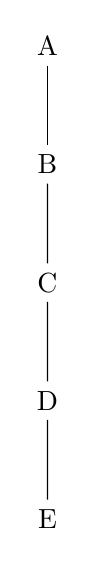
\begin{tikzpicture}
            \node {A}
                child {node {B}
                    child {node {C}
                        child {node {D}
                            child {node {E}}
                        }
                    }
                };
        \end{tikzpicture}
    \end{center}
    \columnbreak
    \begin{center}
        最小內部節點與最大外部節點\\
        external nodes = 2, internal nodes = 3\\
        \vspace{4em}
        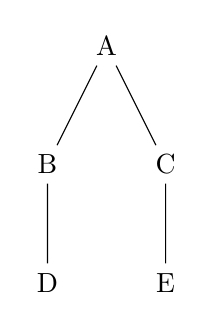
\begin{tikzpicture}
            \node {A}
                child {node {B}
                    child {node {D}}
                }
                child {node {C}
                    child {node {E}}
                };
        \end{tikzpicture}
    \end{center}
    \end{multicols}
    \item PreorderTraversal of a expression tree
    \begin{center}
        $-$ / $\times$ + 3 1 3 + $-$ 9 5 2 + $\times$ 3 $-$ 7 4 6
    \end{center}
    \item Draw the expression tree
    $$\color{red}(\color{blue}(\color{brown}(\color{black}5 + 2\color{brown})\color{black}
        \times\color{brown}(\color{black}2 - 1\color{brown})\color{blue})\color{black}
        /\color{blue}(\color{brown}(\color{black}2 + 9\color{brown})\color{black}
         + \color{brown}(\color{orange}(\color{black}7 - 2\color{orange})\color{black}
         - 1\color{brown})\color{blue})\color{black} \times 8\color{red})$$
    \begin{center}
        \begin{tikzpicture}
            \node {$\times$}
            [level/.style={sibling distance=60mm/#1}]
            [level 2/.style={sibling distance=60mm}]
            [level 3/.style={sibling distance=30mm}]
            [level 4/.style={sibling distance=20mm}]
            child
            {
                node{$\div$}
            child 
            {
                node {$\times$}
                child
                {
                    node {$+$}
                    child {node {5}}
                    child {node {2}}
                }
                child 
                {
                    node {$-$}
                    child {node {2}}
                    child {node {1}}
                }
            }
            child
            {
                node {$+$}
                child 
                {
                    node {$-$}
                    {
                        child {node {2}}
                        child {node {9}}
                    }
                }
                child 
                {
                    node {$-$}
                    {
                        child 
                        {
                            node {$-$}
                            child {node {7}}
                            child {node {2}}
                        }
                        child {node {1}}
                    }
                }
            }
            }
            child
            {
                node{8}
            };
                
        \end{tikzpicture}
    \end{center}
            
\end{enumerate}

\end{CJK*}
\end{document}